%%% TO DO
%  scrivere qualcosa per quanto riguarda le stats su moody lyrics
%  cercare altri dataset
%  trovare come esattamente viene fatto il word embedding 

\documentclass[xcolor=dvipsnames]{beamer}
\usepackage[utf8]{inputenc}
\usepackage{hyperref}
\usepackage[super]{nth} % for 1st, 2nd, etc...
\setbeamertemplate{caption}[numbered] %for figures numbering
\usepackage[export]{adjustbox} %for left and right
\usepackage{siunitx} % for degree symbol

\usetheme{CambridgeUS}

\definecolor{UBCblue}{rgb}{0.04706, 0.13725, 0.26667} % UBC Blue (primary)
\definecolor{UBCgrey}{rgb}{0, 0.46, 0.7} % UBC Grey (secondary)

\setbeamercolor{title}{bg=UBCblue,fg=white}
\setbeamercolor{frametitle}{bg=UBCblue, fg=white}
\setbeamercolor{palette primary}{bg=UBCblue,fg=white} %basso a destra
\setbeamercolor{palette secondary}{fg=UBCblue} %basso al centro
\setbeamercolor{palette tertiary}{bg=UBCgrey,fg=white} %basso e alto a sx 

\setbeamercolor{structure}{fg=UBCblue} % itemize, enumerate, etc
\setbeamercolor{section in toc}{fg=UBCblue} % TOC sections
\setbeamercolor{block title}{bg=UBCgrey!50,fg=black}
\setbeamercolor{block title example}{bg=UBCgrey!50,fg=black}

%------------------------------------------------------------
%This block of code defines the information to appear in the
%Title page
\title[Emotion Patterns in Music Playlists] %optional
{Emotion Patterns in Music Playlists}

%\subtitle{\nth{1} meeting}

\author[Sara, Mario] % (optional)
{Sara Giammusso\inst{1}\inst{2} \and Mario Guerriero \inst{1}\inst{2}}

\institute[EURECOM] % (optional)
{
 \inst{1}
 MSc student in Data Science Department, EURECOM, T\'el\'ecom ParisTech, France\\
  \inst{2}%
 MSc student in Department of Control and Computer Engineering, Politecnico di Torino, Italy
}


\date[2018 March 27] % (optional)
{Second Project meeting}


%End of title page configuration block
%-----------------------------------------------------------



%------------------------------------------------------------
%The next block of commands puts the table of contents at the 
%beginning of each section and highlights the current section:

\AtBeginSection[]
{
  \begin{frame}
    \frametitle{Table of Contents}
    \tableofcontents[currentsection]
  \end{frame}
}
%------------------------------------------------------------


\begin{document}

%The next statement creates the title page.
\frame{\titlepage}

%---------------------------------------------------------
%This block of code is for the table of contents after
%the title page
\begin{frame}
\frametitle{Table of Contents}
\tableofcontents
\end{frame}
%---------------------------------------------------------

\section{Introduction}
%Intoduction
\begin{frame}{Introduction}
\begin{block}{Previously On Sara\&Mario Project...}
In the previous meeting we analyzed the \textbf{state-of-the-art} of text-based Emotion Detection.\\
\end{block}
Next steps:
\begin{itemize}
\item Analyze \textbf{existent} emotion classifiers
\item Research text corpus with \textbf{labeled} emotions
\item Natural language \textbf{processors} and \textbf{embedders}
\item Statistics and \textbf{details} about MoodyLyrics
\end{itemize}



\end{frame}

%Existent emotion classifier
\section{Existent emotion classifiers}

\begin{frame}{Emotion classifiers analysis}
The emotion classifiers APIs we analyzed are: 
\begin{enumerate}
\item IBM Watson NLU
\item IBM Watson Tone Analyzer
\item ParallelDots AI
\item Qemotion
\end{enumerate}
\end{frame}

% IBM Watson: NLU (I)
\begin{frame}{1) IBM Watson: Natural Language Understanding (I)}
Watson is a \textbf{question answering computer} system capable of answering questions posed in \textbf{natural language}, developed by IBM.\cite{p2}
\begin{block}{Cool story}
In 2011, the Watson computer system competed on Jeopardy! against legendary champions Brad Rutter and Ken Jennings winning the first place prize of \$1 million \cite{p2}.
\end{block}
\end{frame}

% IBM Watson: NLU (II)
\begin{frame}{1) IBM Watson: Natural Language Understanding (II)}
\textbf{Natural Language Understanding} is a collection of \textbf{APIs} that allows to:\cite{p1}\\
\begin{itemize}
\item Recognize the \textbf{overall sentiment}, in a scale from negative to positive [-1,1];
\item Detect the \textbf{emotion percentage} between: joy, anger, disgust, sadness, fear;
\item Determine \textbf{keywords} ranked by relevance;
\item Extract \textbf{entities}: people, companies, organizations, cities and other information;
\item Classify content into a \textbf{hierarchical categories};
\item Identify \textbf{general concepts} that may not be directly referenced in the text;
\item Distinguish the \textbf{semantic roles} parsing sentences into subject, action and object.
\end{itemize}
\end{frame}

%\setbeamerfont{caption}{series=\normalfont,size=\fontsize{4}{6}} 
% IBM Watson NLU: DEMO (I)
\begin{frame}{1) IBM Watson NLU: Demo (I)}
Results obtained analyzing \textbf{Oasis - Wonderwall} lyrics (I).
\begin{columns}
\column{0.7\textwidth}
\begin{figure}
	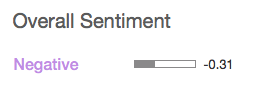
\includegraphics[scale=0.3,left]{./images/sentiment}
	%\caption{Overall Sentiment}
\end{figure}
\begin{figure}
	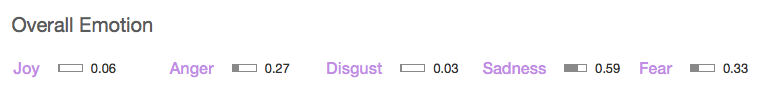
\includegraphics[scale=0.3,left]{./images/emotion}
	%\caption{Overall Emotion}
\end{figure}
\begin{figure}
	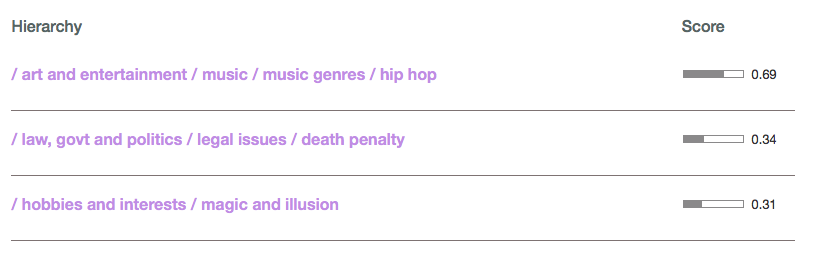
\includegraphics[scale=0.3,left]{./images/categories}
\end{figure}
\column{0.3\textwidth}
\begin{figure}
	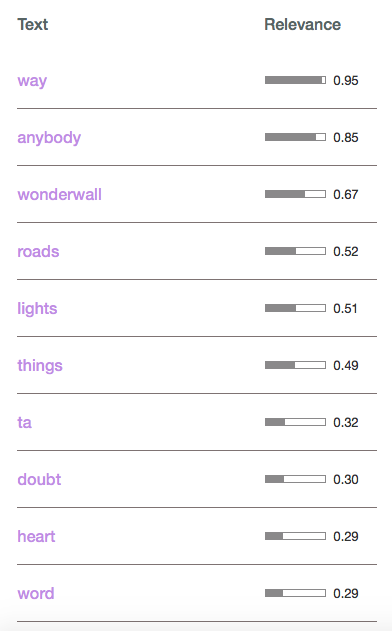
\includegraphics[scale=0.25,left]{./images/keywords}
\end{figure}
\end{columns}
\end{frame}

% IBM Watson NLU: DEMO (II)
\begin{frame}{1) IBM Watson NLU: Demo (II)}
Results obtained analyzing \textbf{Oasis - Wonderwall} lyrics (II).
\begin{columns}
\column{0.5\textwidth}
\begin{figure}
	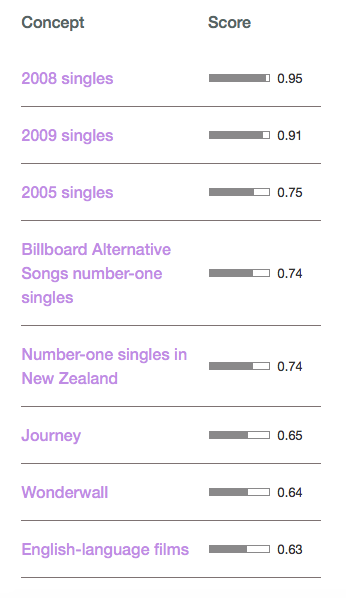
\includegraphics[scale=0.3]{./images/concept}
\end{figure}
\column{0.5\textwidth}
\begin{figure}
	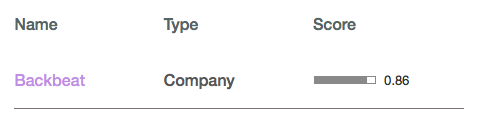
\includegraphics[scale=0.3]{./images/entities}
\end{figure}
\begin{figure}
	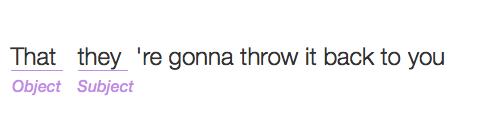
\includegraphics[scale=0.3]{./images/roles}
\end{figure}
\end{columns}
\end{frame}

%IBM Watson: Tone Analyzer
\begin{frame}{2) IBM Watson: Tone Analyzer}
It uses linguistic analysis to detect joy, fear, sadness, anger, analytical, confident and tentative tones found in text. \cite{p3}
\begin{block}{Possible sources}
Tweets, Online Review, Email message, your own text.
\end{block}
It uses both:
\begin{itemize}
\item \textbf{the document level}: to get a sense of the overall tone 
\item and the \textbf{sentence level}: to identify specific areas of your content where tones are the strongest.
\end{itemize}
The results obtained with \textbf{Oasis - Wonderwall} are identical to the ones obtained from \textbf{IBM Watson: NLU}
\end{frame}

%ParallelDots APIs: Demo
\begin{frame}{3) ParallelDots APIs: Demo}
Their \textbf{Emotion Analysis classifier} is trained on their proprietary dataset and tells whether the underlying emotion behind a message is: \textbf{Happy, Sad, Angry, Fearful, Excited, Funny or Sarcastic}.\cite{p4}
\\The result obtained analyzing \textbf{Oasis - Wonderwall} lyrics is showed in the following figure. 
\begin{figure}
	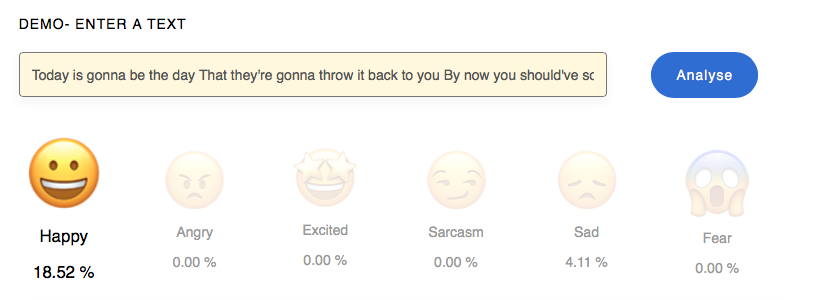
\includegraphics[scale=0.3]{./images/pd_wonderwall}
	\caption{Output for Oasis - Wonderwall}
\end{figure}
\end{frame}

%QEmotion
\begin{frame}{4) Qemotion}
Qemotion detects the main emotion of the speech and will define the corresponding emotion in terms of \textbf{temperature} (literally temperature) \cite{p5}.
\begin{itemize}
\item From \ang{31}C to \ang{40}C $\rightarrow$ Happiness
\item From \ang{21}C to \ang{30}C $\rightarrow$ Surprise
\item From \ang{11}C to \ang{20}C $\rightarrow$ Calm
\item From \ang{6}C to \ang{10}C $\rightarrow$ Fear
\item From \ang{-5}C to \ang{5}C $\rightarrow$ Sadness and Disappointment
\item From \ang{-14}C to \ang{-6}C $\rightarrow$ Anger
\item From \ang{-20}C to \ang{-15}C $\rightarrow$ Disgust
\end{itemize}
\end{frame}

% Note about plans
\begin{frame}{Note about plans}
\begin{block}{Note}
None of these APIs is free, however they offer a limited number of free API calls
\end{block}
\end{frame}

% NLP libraries
\section{NLP libraries}

% NLP libraries
\begin{frame}{NLP libraries}
The main NLP libraries are:
\begin{enumerate}
\item NLTK
\item TextBlob
\item Stanford's CoreNLP
\item SpaCy
\end{enumerate}
\end{frame}

%1) NLTK: Natural Language Toolkit
\begin{frame}{1) NLTK: Natural Language Toolkit}
Recommend only as an \textbf{education and research} tool.\\
Pros:
\begin{itemize}
\item its \textbf{modularized} structure makes it excellent for learning and exploring NLP concepts;
\item over 50 corpora and lexicons, 9 stemmers, and dozens of algorithms to choose from (also a con);
\end{itemize}
Cons:
\begin{itemize}
\item \textbf{Heavy} and it has a \textbf{steep} learning curve;
\item \textbf{slow} and not production-ready.
\end{itemize}
See also \textbf{NTLK Book} \cite{p6}.
\end{frame}

%2) TextBlob
\begin{frame}{2) TextBlob}
Built on top of NLTK.\\
Pros:
\begin{itemize}
\item More intuitive;
\item Gentle learning curve.
\end{itemize}
See also \textbf{``NLP Basics with TextBlob"} \cite{p7}.
\end{frame}

%3) Stanford's CoreNLP
\begin{frame}{3) Stanford's CoreNLP}
Java library with Python wrappers.\\
Pros: 
\begin{itemize}
\item fast;
\item support for several major languages.
\end{itemize}
\end{frame}

% 4) SpaCy
\begin{frame}{4) SpaCy}
It's a new NLP library  designed to be \textbf{fast}, streamlined, and production-ready.\\
Pros:
\begin{itemize}
\item \textbf{minimal}: it doesn't flood you with a lot of options
\item its philosophy is to only present \textbf{one algorithm} (the best one) for each purpose.
\end{itemize}
Cons:
\begin{itemize}
\item it's \textbf{new}, so its support community is not as large as some other libraries
\item it currently only supports English.
\end{itemize}
See also \textbf{``Intro to NLP with SpaCy"} \cite{p8}. 
\end{frame}

% Word Embeddings
\begin{frame}{Word Embeddings}
Word embeddings are a set of feature learning techniques which map \textbf{words} or phrases from the vocabulary to vectors of \textbf{real numbers}. \\
These techniques map \textbf{sparse} word vectors into \textbf{continuous} space based on the surrounding context.\\
\begin{Example}
If `\textbf{``salt"} and \textbf{``seasoning"} appear within the same context, the model will indicate that ``salt" is conceptually closer to ``seasoning," than, say, ``chair." 
\end{Example}
There are 2 main Embedding libraries:
\begin{enumerate}
\item Word2Vec
\item FastText
\end{enumerate}
\end{frame}

% Word2Vec VS FastText (I)
\begin{frame}{Word2Vec VS FastText (I)}
\begin{block}{Main difference}
\textbf{Word2vec} treats each word in corpus like an \textbf{atomic entity} and generates a vector for each word.\\
\textbf{FastText} treats each as \textbf{composed} of character ngrams, so the vector for a word is made of the sum fo this character n grams.
\end{block}
\begin{Example}
 The word vector ``apple" is a sum of the vectors of the n-grams ``ap", ``app", ``appl", ``apple", ``ppl", ``pple", ``pple", ``ple", ``le" (assuming hyperparameters for smallest ngram[minn] is 3 and largest ngram[maxn] is 6).
\end{Example}
\end{frame}
% Word2Vec VS FastText (II)
\begin{frame}{Word2Vec VS FastText (II)}
This difference manifests as follows:
\begin{enumerate}
\item \textbf{Rare words}: even if words are rare their character n grams are still shared with other words - hence the embeddings with FastText can still be good.
\item \textbf{Out of vocabulary words}: FastText can construct the vector for a word from its character n grams even if word doesn't appear in training corpus.
\item \textbf{Hyperparameters choice}: FastText requires to choose the the minimum and maximum n-gram sizes, and this directly impacts:
	\begin{itemize}
	\item computation time
	\item memory requirements
	\end{itemize}

\end{enumerate}
\end{frame}

%Lyrics Downloader Script 1
\section{Lyrics Downloader Script}
\begin{frame}{lyrics\_downloader.py (1)}

We wrote a Python script for downloading lyrics. We used:
\begin{itemize}
\item MoodyLyrics to get songs information (artist, title and emotion)
\item LyricWikia to download the lyrics
\end{itemize}

\end{frame}

%Lyrics Downloader Script 2
\begin{frame}{lyrics\_downloader.py (2)}

Our script produces in output:
\begin{itemize}
\item A folder containing lyrics in files named: \textit{EMOTION\_ARTIST\_TITLE-OF-SONG}
\item A log file in which we keep track of the errors we found
\end{itemize}

\end{frame}

%References

\section{References}
\begin{frame}{References}
\setbeamertemplate{bibliography item}[text]
 \begin{thebibliography}{99} % Beamer does not support BibTeX so references must be nserted manually as below
\bibitem{p1} IBM Watson: Natural Language Understanding APIs
\footnotesize \url{https://www.ibm.com/watson/services/natural-language-understanding/}

\bibitem{p2} IBM Watson - Wikipedia
\footnotesize \url{https://en.wikipedia.org/wiki/Watson_(computer)}

\bibitem{p3} IBM Watson: Tone Analyzer
\footnotesize\url{https://en.wikipedia.org/wiki/Watson_(computer)}

\bibitem{p4} ParallelDots APIs
\footnotesize \url{https://tone-analyzer-demo.ng.bluemix.net/}

\bibitem{p5} Qemotion
\footnotesize \url{http://www.qemotion.com/demo.php}

\bibitem{p6} NTLK Book
\footnotesize \url{http://www.nltk.org/book/}

\bibitem{p7} Natural Language Basics with TextBlob
\footnotesize\url{http://rwet.decontextualize.com/book/textblob/}

\bibitem{p8} Intro to NLP with SpaCy
\footnotesize\url{https://nicschrading.com/project/Intro-to-NLP-with-spaCy/}

\end{thebibliography}

\end{frame}
%---------------------------------------------------------

\end{document}
